\input{configuration}

\def\ojoin{\setbox0=\hbox{$\bowtie$}%
  \rule[-.02ex]{.25em}{.4pt}\llap{\rule[\ht0]{.25em}{.4pt}}}
\def\leftouterjoin{\mathbin{\ojoin\mkern-5.8mu\bowtie}}

\title{Tutorial 9 --- Isolation and Recovery }

\author{Richard Wong \\ \small \texttt{rk2wong@edu.uwaterloo.ca}}
\institute{Department of Electrical and Computer Engineering \\
  University of Waterloo}
\date{\today}


\begin{document}

\begin{frame}
  \titlepage

\end{frame}


\begin{frame}
\frametitle{Exercise 9-1}

For the following transaction schedule, fill in the RW-timestamps for data items $a$ and $b$, assuming we use the simple timestamp-ordering protocol.

How would the answer change if we used the Thomas Write Rule?

\begin{center}
\begin{tabular}{ | c c c || c c c c | }
  \hline
  $T_1$ & $T_2$ & $T_3$ & $TS_r(a)$ & $TS_w(a)$ & $TS_r(b)$ & $TS_w(b)$ \\
  \hline
  $r_a$ &       &       &           &           &           &           \\
        & $r_b$ &       &           &           &           &           \\
        &       & $r_a$ &           &           &           &           \\
  $w_a$ &       &       &           &           &           &           \\
        & $r_a$ &       &           &           &           &           \\
        &       & $w_b$ &           &           &           &           \\
  $r_b$ &       &       &           &           &           &           \\
        & $w_b$ &       &           &           &           &           \\
        &       & $w_a$ &           &           &           &           \\
  \hline
\end{tabular}
\end{center}

\end{frame}



\begin{frame}
\frametitle{Exercise 9-1 Solution}


\begin{center}
\begin{tabular}{ | c c c || c c c c | }
  \hline
  $T_1$ & $T_2$ & $T_3$ & $TS_r(a)$ & $TS_w(a)$ & $TS_r(b)$ & $TS_w(b)$ \\
  \hline
  $r_a$ &       &       & 1         &           &           &           \\
        & $r_b$ &       &           &           & 2         &           \\
        &       & $r_a$ & 3         &           &           &           \\
  $w_a$ &       &       &           & 1<3, abort $T_1$ &    &           \\
        & $r_a$ &       & 3         &           &           &           \\
        &       & $w_b$ &           &           &           & 3         \\
  $r_b$ &       &       &           &           &           &           \\
        & $w_b$ &       &           &           &           & 2<3, abort $T_2$ \\
        &       & $w_a$ &           & 3         &           &           \\
  \hline
\end{tabular}
\end{center}

If we used the Thomas Write Rule, $T_2$ would not need to abort just because it wanted to write a value that would have already been overwritten by $T_3$, and the write would have been ignored instead.

\end{frame}


\begin{frame}
\frametitle{Exercise 9-2}

Under what conditions does the phantom read phenomenon occur?

\end{frame}


\begin{frame}
\frametitle{Exercise 9-2 Solution}

Phantom reads happen when reads and writes conflict on unisolated, non-tuple data.

e.g. \\
Query 1: SELECT a COUNT of the number of Math professors at Waterloo. \\
Query 2: INSERT a Waterloo Math professor.

Transaction 1: Run Query 1 twice. \\
Transaction 2: Run Query 2 once.

This poses a problem for serialized isolation. The result of the SELECT will differ based on whether it runs before or after the INSERT. If the SELECTs happen on either side of the INSERT, then Transaction 1 will see inconsistent information. In serialized isolation, each transaction should be able to assume that it is the only transaction running at a time.

This is allowed to happen since we can't lock rows that do not exist (yet). We fix this with a protocol that locks index leaf nodes, under the assumption that every query uses an index.

\end{frame}


\begin{frame}
\frametitle{Exercise 9-3}

Suppose we need to recover from a system failure, and have the transaction log below.

Assuming we use an immediate update protocol with checkpointing, what log entries does the recovery system need to add to restore the database to a consistent state?

\begin{center}
\begin{tabular}{ | l | c c c c | c | }
  \hline
  action & transaction & item & val & val' & flags \\
  \hline
  start & $T_1$ &   &   &   &           \\
  write & $T_1$ & a & 1 & 2 &           \\
  write & $T_1$ & a & 2 & 3 &           \\
  checkpoint & [$T_1$] &   &   &   &           \\
  want to abort & $T_1$ &   &   &   &           \\
  write & $T_1$ & a & - & 2 & redo-only \\
  start & $T_2$ &   &   &   &           \\
  write & $T_2$ & b & 5 & 6 &           \\
  write & $T_2$ & b & 6 & 7 &           \\
  (system failure) &       &   &   &   &           \\
  \hline
\end{tabular}
\end{center}

\end{frame}


\begin{frame}
\frametitle{Exercise 9-3 Solution}

\begin{center}
\begin{tabular}{ | l | c c c c | c | }
  \hline
  action & transaction & item & val & val' & flags \\
  \hline
  start & $T_1$ &   &   &   &           \\
  write & $T_1$ & a & 1 & 2 &           \\
  write & $T_1$ & a & 2 & 3 &           \\
  checkpoint & [$T_1$] &   &   &   &           \\
  want to abort & $T_1$ &   &   &   &           \\
  write & $T_1$ & a & - & 2 & redo-only \\
  start & $T_2$ &   &   &   &           \\
  write & $T_2$ & b & 5 & 6 &           \\
  write & $T_2$ & b & 6 & 7 &           \\
  (system failure) &       &   &   &   &           \\
  \hline
  write & $T_2$ & b & - & 6 & redo-only \\
  write & $T_2$ & b & - & 5 & redo-only \\
  abort & $T_2$ &   &   &   &           \\
  write & $T_1$ & a & - & 1 & redo-only \\
  abort & $T_1$ &   &   &   &           \\
  \hline
\end{tabular}
\end{center}

\end{frame}


\begin{frame}
\frametitle{Exercise 9-4}

Where do the following recovery protocols belong in the table below?

\begin{enumerate}
  \item deferred update
  \item immediate update (\textit{can} persist prior to commit)
  \item strict immediate update (persist changes immediately)
\end{enumerate}

\begin{center}
\begin{tabular}{ | l | c | c | }
  \hline
          & redo & no-redo \\
  \hline
  undo    &      &         \\
  \hline
  no-undo &      &         \\
  \hline
\end{tabular}
\end{center}

\end{frame}


\begin{frame}
\frametitle{Exercise 9-4 Solution}

\begin{center}
\begin{tabular}{ | l | c | c | }
  \hline
          & redo & no-redo \\
  \hline
  undo    & immediate update & strict immediate update \\
  \hline
  no-undo & deferred update & (this is called giving up) \\
  \hline
\end{tabular}
\end{center}

\end{frame}


\begin{frame}
\frametitle{Exercise 9-5}
  What data is logged in order for the ARIES protocol to restore from a checkpoint?
\end{frame}


\begin{frame}
\frametitle{Exercise 9-5 Solution}
  In an ARIES checkpoint, the transaction table (TT) and dirty page table (DPT) at the time of checkpoint are written to the log.

  The TT needs to know the IDs of the active transactions, the last LSN associated with each transaction, and the status of each transaction.

  The DPT needs to know the IDs of the dirty pages (those that require updates), and the most recent (greatest) LSN associated with each page.

  Recall that LSNs are written only for:
  \begin{enumerate}
    \item write an update
    \item commit transaction
    \item abort transaction
    \item undo an update
    \item end transaction
  \end{enumerate}
\end{frame}


\begin{frame}
\frametitle{Exercise 9-6}
  Suppose a checkpoint is made between LSN 7 and 8 in the following schedule.

  What data is stored in the transaction table and the dirty page table?

  Where should the REDO phase start scanning for operations?

  \begin{center}
  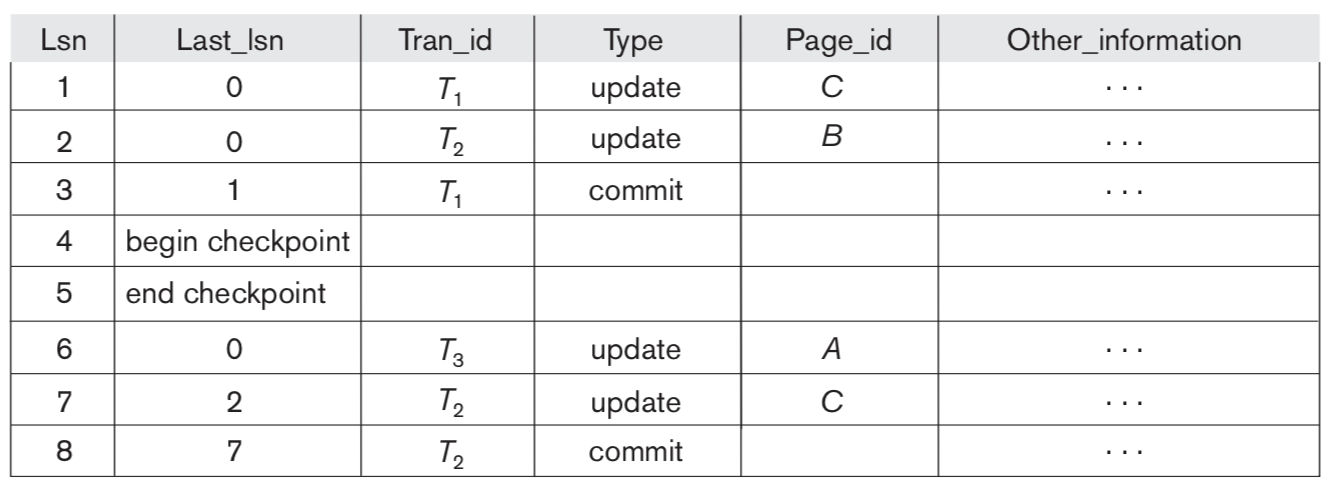
\includegraphics[width=0.85\textwidth]{images/aries-1}\\
  \end{center}
\end{frame}


\begin{frame}
\frametitle{Exercise 9-6 Solution (1/2)}

Recall:

The transaction table contains all transactions that were active at the time of the checkpoint, the LSN of the most recent log entry for each transaction, and the status of each transaction (in progress, committing, aborting).

The dirty page table holds the pages that have been modified and have not yet been written (persisted) to disk, and the first LSN that caused an update in each page.

\end{frame}


\begin{frame}
\frametitle{Exercise 9-6 Solution (2/2)}

Transaction table:
\begin{center}
\begin{tabular}{ | l | c | c | }
  \hline
  transactionId & lastLSN & status \\
  \hline
  $T_1$ & 3 & commit \\
  \hline
  $T_2$ & 7 & in progress \\
  \hline
  $T_3$ & 6 & in progress \\
  \hline
\end{tabular}
\end{center}

Dirty page table:
\begin{center}
\begin{tabular}{ | l | c | }
  \hline
  transactionId & lastLSN \\
  \hline
  C & 1 \\
  \hline
  B & 2 \\
  \hline
  A & 6 \\
  \hline
\end{tabular}
\end{center}

\end{frame}



\begin{frame}
\frametitle{Exercise 9-7}
  Why is it important for the ARIES protocol to look for the most recent \textit{end-checkpoint} log record as opposed to the most recent \textit{start-checkpoint} log record during its analysis phase (finding TT and DPT at last checkpoint)?
\end{frame}


\begin{frame}
\frametitle{Exercise 9-7 Solution}
  The \textit{end-checkpoint} log entry tells us that the TT and DPT have been fully written and that the checkpoint completed successfully. The log entry also contains the LSN of the corresponding \textit{start-checkpoint} log entry, which marks where to start reading the TT and DPT.
\end{frame}


\end{document}
